\documentclass[11pt, a4]{article}
\newcommand{\lotteryset}{\mathcal{L}}
\newcommand{\outcomeset}{\mathcal{X}}
\usepackage{amssymb}
\usepackage{enumitem}
\usepackage{amsmath}
\usepackage{tfrupee}
\usepackage{pgfplots}
\usepackage{tikz}
\usepackage{enumitem}
\usepackage{multirow}
\usepackage{fancyhdr}
\usepackage{lastpage}
\usepackage[export]{adjustbox}
\usepackage{wrapfig}
\usepackage[english]{babel}
\usepackage{amsthm}
\usepackage{multirow}
\usepackage{wrapfig,lipsum,booktabs}
\usepackage{graphicx}
\usepackage{subcaption} 
\usepackage{float}
\usepackage{hyperref}

\topmargin -0.0in
% \textheight 11in
\oddsidemargin .5in
\evensidemargin 0.0in
\textwidth 5.5in

\begin{document}
	\pagestyle{fancy}
	\fancyhead{}\fancyfoot{}
	\fancyhead[L]{PA-2 Report}
	\fancyhead[C]{\thepage ~of \pageref{LastPage}}
	\fancyhead[R]{EE25S009}
	\author{Ritabrata Mandal\\ EE25S009}
	\title{EE5176: Computational Photography\\Programming Assignment-2: Motion Deblurring Report}
	\maketitle
	
	\medskip
	\newpage
	\begin{enumerate}[label=\arabic*.,start=0]
		\item \textbf{Introduction}\\
		This assignment explores imaging scenarios that result in motion blur and examines various methods to reduce it. 
		\begin{enumerate}
			\item \textbf{Problem Description}\\
			 Motion blur can occur when the camera moves while capturing a static scene, when an object in the scene is moving, or when both effects are present. Even with knowledge of the blur kernel, deblurring remains a challenging task in conventional photography. Assuming a 1D blur with a box-shaped kernel, its frequency-domain representation is a sinc function. A straightforward approach to deblurring is to divide the frequency response of the blurred image by that of the transfer function, and then estimate the deblurred image using the inverse transform. However, this method suffers from noise amplification, especially when the transfer function approaches zero. An additional complication arises with non-uniform blur, which often occurs when multiple objects move within the scene along with camera motion. Estimating separate blur kernels for each object requires segmentation, a difficult and error-prone task. For this reason, uniform blurring across the image is desirable, as it avoids the need for segmentation.  
			 \item \textbf{Implementation}\\
			 The implementation has been carried out and tested in python 3.12.10. All processed images generated during this assignment are available in the GitHub repository under the  			 \href{https://github.com/RitabrataMandal/EE5176/tree/master/Assignments/Assignment2/output}{\texttt{output}} folder.
			 \item \textbf{Running the Code}\\
			 To execute the assignment, navigate to the \href{https://github.com/RitabrataMandal/EE5176/tree/master/Assignments/Assignment2}{\texttt{Assignment2}} folder, run the \texttt{main.ipynb} file.
		\end{enumerate}
		\item \textbf{Motion Deblurring with Conventional Camera}\\
		We are given a clean image of a scene having $M$ and $N$ columns ($\texttt{fist.png}$) shown in Figure \ref{fig:original_image}. We capture the scene using a static conventional camera with the aperture kept open for the full exposure time. The exposure time is $52$ seconds. For simplicity, consider that the camera captures the scene at times $t=0,\cdots,51$. At time $t=0,$ the image has zero translation. Then, the whole image as seen by the camera moves at 1 pixel per second to the right (horizontal translation).
		\begin{figure}[H]
			\centering
			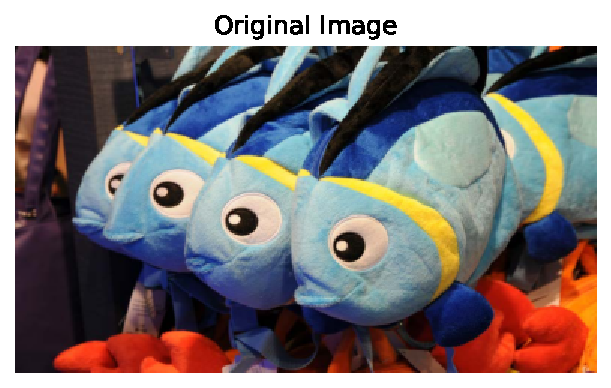
\includegraphics[width=0.7\linewidth]{../output/original.pdf}
			\caption{Original Image}
			\label{fig:original_image}
		\end{figure}
		\begin{enumerate}
			\item  \textbf{Generating the Blurred Image}\\
			We generate the blurred image having $M$ and $N+1$ columns captured by the camera. We generate the translated versions of the image for $t=\{0,1\cdots,51\}$ and average them. We add Gaussian noise mean $0$ and standard deviation $1$ (with respect to the maximum intensity of $255$) from \texttt{gaussNoise.mat}. The blurred image is shown in Figure \ref{fig:blurred_conventional}.
			\begin{figure}[H]
				\centering
				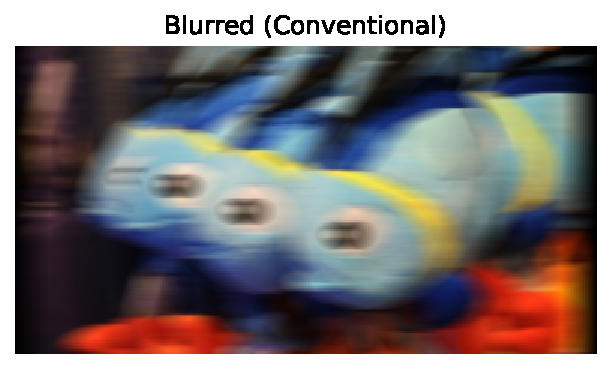
\includegraphics[width=0.7\linewidth]{../output/blurred_conventional.pdf}
				\caption{Blurred image with conventional camera}
				\label{fig:blurred_conventional}
			\end{figure}
			\item \textbf{Blur Matrix}\\
			We form the blur matrix $A$ of size $(N+51)\times N$ corresponding to the horizontal translation described above. This matrix will be a Toeplitz matrix. Figure \ref{fig:toeplitz_matrix_conventional} shows the matrix $A$.
			\begin{figure}[H]
				\centering
				
\includegraphics[width=0.6\linewidth]{../output/toeplitz_matrix_convemtional.pdf}
				\caption{Toeplitz matrix(conventional)}
				\label{fig:toeplitz_matrix_conventional}
			\end{figure}
			\item \textbf{Least Squares Deblurring \& RMSE}\\
			We deblur the noisy image using the least squares and the generated blur matrix $A$. We perform the operation on each channel of the image. If the blurred image channel given by $y$, the reconstructed image channel estimate $\hat{x}$ is given by 
			\begin{align*}
				\hat{x}=yA\left(A^TA\right)^{-1}
			\end{align*}
			Where $A$ is blur(toeplitz) matrix. Figure \ref{fig:reconstructed_conventional} shows the resulting deblurred image. The RMSE between the original image and deblurred image is $0.33359.$
			\begin{figure}[H]
				\centering
				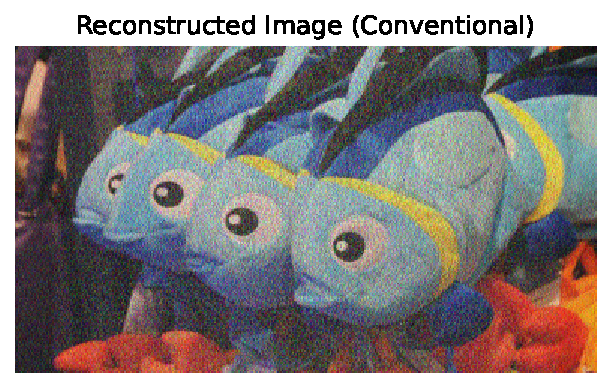
\includegraphics[width=0.7\linewidth]{../output/reconstructed_conventional.pdf}
				\caption{Reconstructed image(conventional)}
				\label{fig:reconstructed_conventional}
			\end{figure}
			\item \textbf{Observation \& Results}\\
			In the deblurred image, a significant amount of noise is visible. This occurs because the pseudo-inverse of the A matrix amplifies the high-frequency components, which in turn amplifies the noise. As a result we see the RMSE of the original image and the reconstructed image is not zero.
		\end{enumerate}
		\item \textbf{Motion Deblurring with Flutter Shutter}\\
		With the same setup as in the previous section, we use a flutter shutter camera with these $2$ codes:
		\begin{enumerate}[label=(\roman*)]
			\item $1010000111000001010000110011110111010111001001100111$
			\item $1010101010101010101010101010101010101010101010101010$
		\end{enumerate}
		where each bit represents one second of the exposure time.
		\begin{enumerate}
			\item \textbf{Generating the Blurred Image}\\
			We generate blurred images with noise (similar to those captured by a conventional camera) using the exposure codes provided above. Figure \ref{fig:blurred_seq_1} and Figure \ref{fig:blurred_seq_2} show the resulting images corresponding to the two code sequences.
			\begin{figure}[H]
				\centering
				\resizebox{\linewidth}{!}{
					\begin{tabular}{c}
						\begin{subfigure}[h]{1\linewidth}
							\centering
							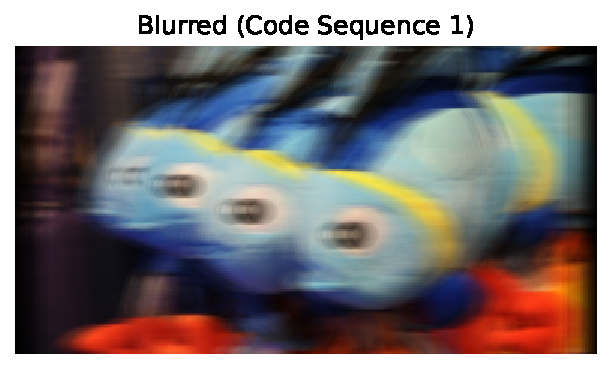
\includegraphics[width=.7\linewidth]{../output/blurred_seq_1.pdf}
							\caption{Blurred(Code Sequence 1)}
							\label{fig:blurred_seq_1}
						\end{subfigure} \\
						\begin{subfigure}[h]{1\linewidth}
							\centering
							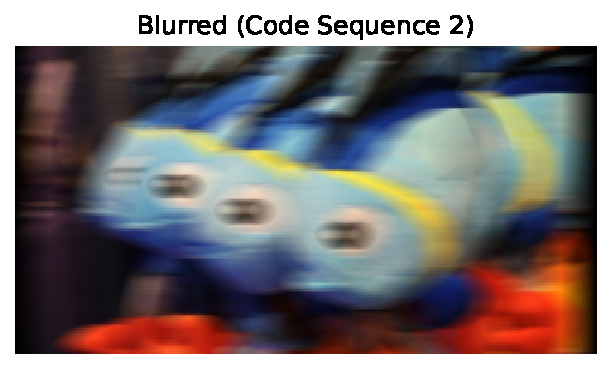
\includegraphics[width=.7\linewidth]{../output/blurred_seq_2.pdf}
							\caption{Blurred(Code Sequence 2)}
							\label{fig:blurred_seq_2}
						\end{subfigure}
					\end{tabular}
				}
				\caption{Blurred image with flutter shutter camera}
				\label{fig:blurred_flutter}
			\end{figure}
			\item \textbf{Blur Matrix}\\
			We construct the blur matrices $A$ in the same manner as in the conventional camera case. Figure \ref{fig:toeplitz_matrix_seq_1} illustrates the matrix $A$ for code sequence 1, while Figure~\ref{fig:toeplitz_matrix_seq_2} shows the corresponding matrix for code sequence 2.
			\begin{figure}[H]
				\centering
				\resizebox{\linewidth}{!}{
					\begin{tabular}{c}
						\begin{subfigure}[h]{1\linewidth}
							\centering
							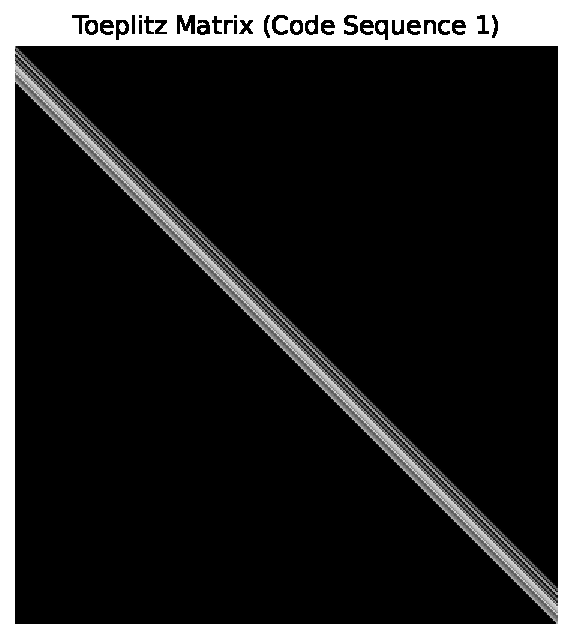
\includegraphics[width=.7\linewidth]{../output/toeplitz_matrix_seq_1.pdf}
							\caption{Blur matrix(Code Sequence 1)}
							\label{fig:toeplitz_matrix_seq_1}
						\end{subfigure} \\
						\begin{subfigure}[h]{1\linewidth}
							\centering
							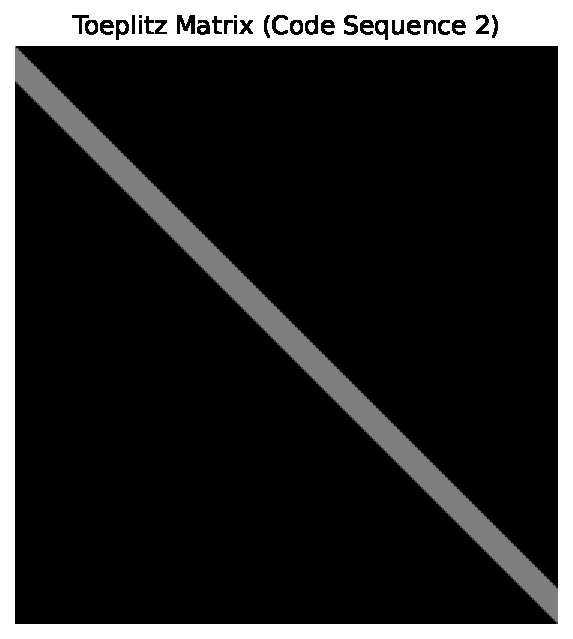
\includegraphics[width=.7\linewidth]{../output/toeplitz_matrix_seq_2.pdf}
							\caption{Blur matrix(Code Sequence 2)}
							\label{fig:toeplitz_matrix_seq_2}
						\end{subfigure}
					\end{tabular}
				}
				\caption{Blurred matrices with different code sequence}
				\label{fig:toeplitz_matrix_seq}
			\end{figure}
			\item \textbf{Frequency Response}\\
			 We compare the frequency responses of the DFTs corresponding to the conventional and flutter shutter codes, using the first column of the respective $A$ matrices. The magnitude in decibels is plotted in Figure \ref{fig:dfts}. The frequency response of the flutter shutter is clearly more desirable, as it does not exhibit dips caused by zeros and does not show a significant reduction in magnitude at higher frequencies. This implies that images obtained using the flutter shutter are easier to deblur compared to those from the conventional case. Moreover, due to the absence of zeros, we do not expect the noise in the deblurred image to be amplified as it is in the conventional camera.
			 \begin{figure}[H]
			 	\centering
			 	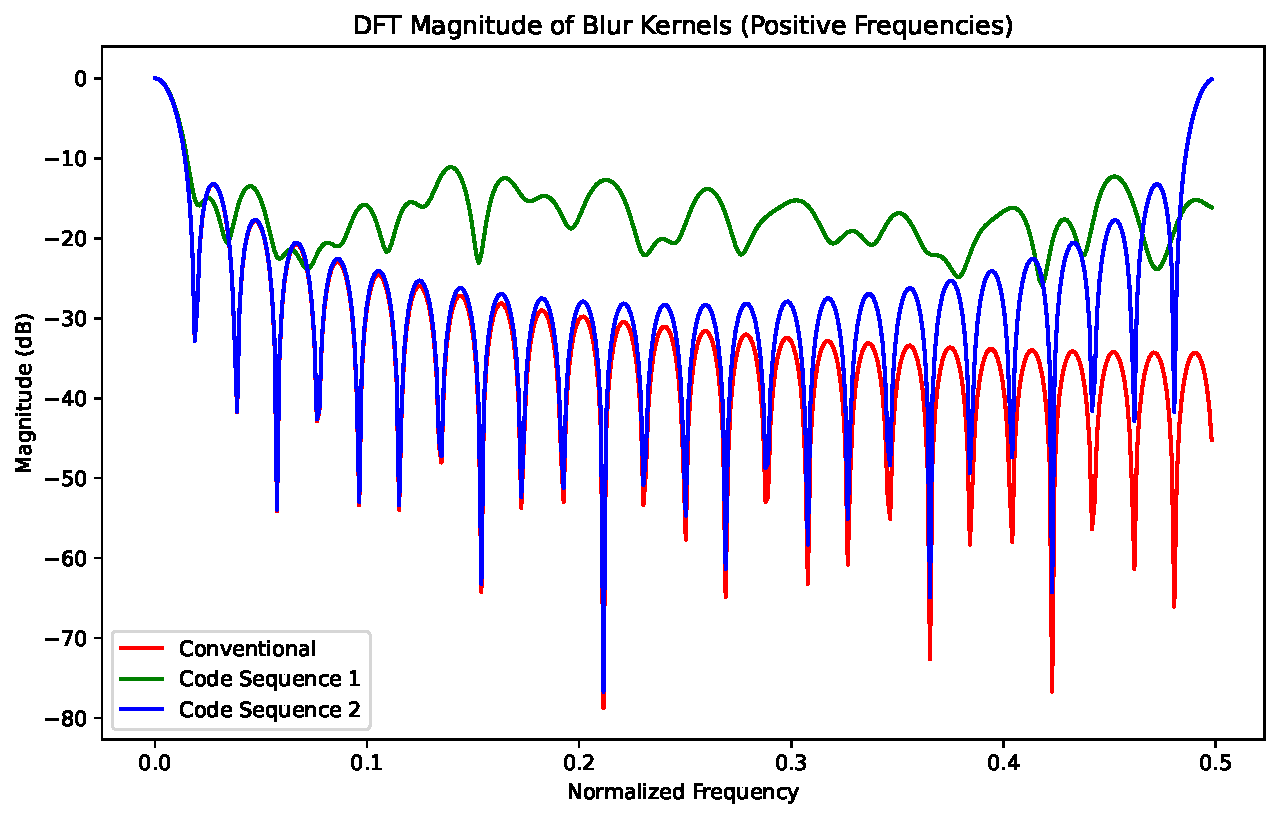
\includegraphics[width=0.7\linewidth]{../output/dft_magnitude_comparison.pdf}
			 	\caption{DFT Magnitude of Blur Kernels}
			 	\label{fig:dfts}
			 \end{figure}
			 \item \textbf{Least Squares Deblurring}\\
			 Similar to the conventional case, we estimate the deblurred image from the $A$ matrices. Figure \ref{fig:reconstructed_seq_1} and Figure \ref{fig:reconstructed_seq_2} show the reconstructed images obtained using the least squares method.
			 \begin{figure}[H]
			 	\centering
			 	\resizebox{\linewidth}{!}{
			 		\begin{tabular}{c}
			 			\begin{subfigure}[h]{1\linewidth}
			 				\centering
			 				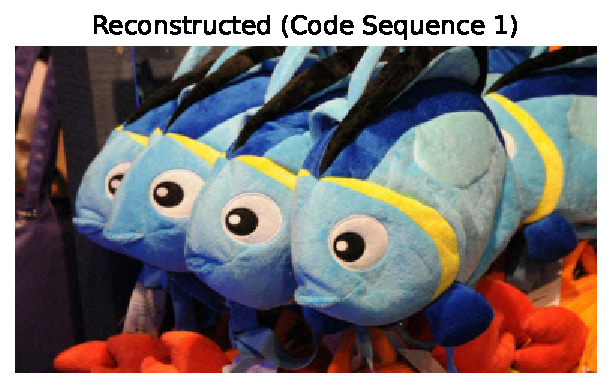
\includegraphics[width=.7\linewidth]{../output/reconstructed_seq_1.pdf}
			 				\caption{Reconstructed(Code Sequence 1)}
			 				\label{fig:reconstructed_seq_1}
			 			\end{subfigure} \\
			 			\begin{subfigure}[h]{1\linewidth}
			 				\centering
			 				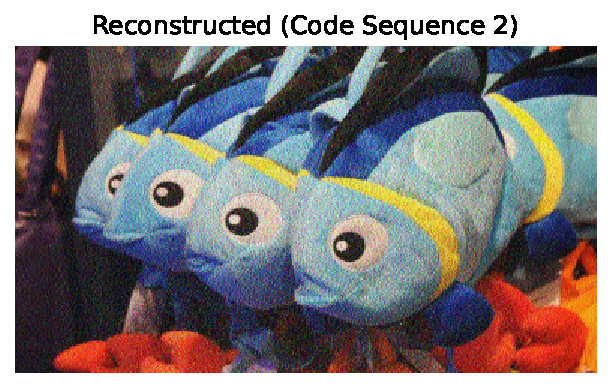
\includegraphics[width=.7\linewidth]{../output/reconstructed_seq_2.pdf}
			 				\caption{Reconstructed(Code Sequence 2)}
			 				\label{fig:reconstructed_seq_2}
			 			\end{subfigure}
			 		\end{tabular}
			 	}
			 	\caption{Reconstructed images}
			 	\label{fig:reconstucetd_flutter}
			 \end{figure}
			 \item \textbf{RMSE \& result comparison}\\
			 For the reconstructed image using code sequence 1, we observe less noise compared to code sequence 2. This is because the DFT of the first sequence is more broadband, leading to reduced amplification of the Gaussian noise added to the blurred image. The RMSE values also support this observation: 0.033 for code sequence 1 versus 0.2033 for code sequence 2.
			\item \textbf{Reconstruction without noise added}\\
			In this case, we don't add Gaussian noise to the image during deblurring and perform the same deblurring procedure as before. Figure \ref{fig:blurred_conventioanl_without_noise}, Figure \ref{fig:blurred_seq_1_without_noise}, and Figure \ref{fig:blurred_seq_2_without_noise} show the blurred images obtained with the conventional camera, flutter shutter code sequence 1, and code sequence 2, respectively. Similarly, Figure \ref{fig:reconstructed_conventioanl_without_noise}, Figure \ref{fig:reconstructed_seq_1_without_noise}, and Figure \ref{fig:reconstructed_seq_2_without_noise} present the reconstructed images for the conventional camera, flutter shutter with code sequence~1, and code sequence 2, respectively. Since the blurred images do not contain noise in this case, the differences between the reconstructed images using the two code sequences are very subtle.
			
			\begin{figure}[H]
				\centering
				\resizebox{1\linewidth}{!}{
					\begin{tabular}{ccc}
						\begin{subfigure}[h]{1\linewidth}
							\centering
							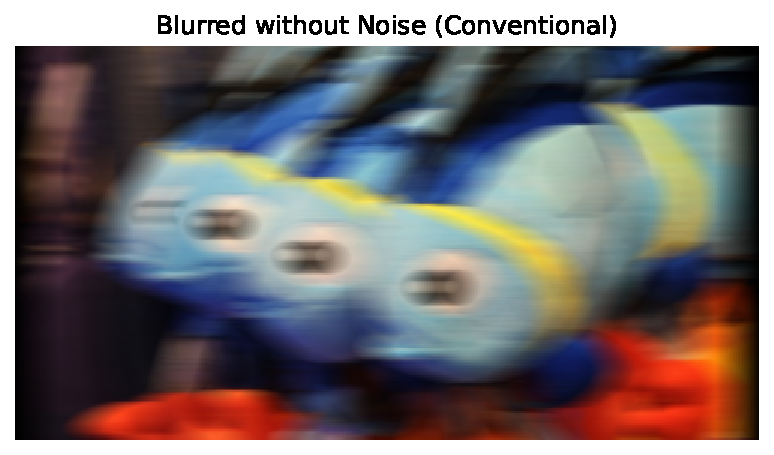
\includegraphics[width=1\linewidth]{../output/blurred_conventional_without_noise.pdf}
							\caption{Blurred without noise(Conventional)}
							\label{fig:blurred_conventioanl_without_noise}
						\end{subfigure} &
						\begin{subfigure}[h]{1\linewidth}
							\centering
							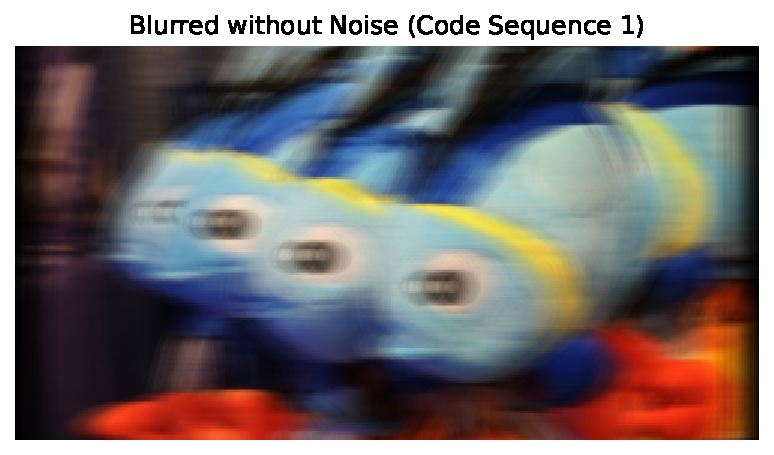
\includegraphics[width=1\linewidth]{../output/blurred_seq_1_without_noise.pdf}
							\caption{Blurred without noise(Code Sequence 1)}
							\label{fig:blurred_seq_1_without_noise}
						\end{subfigure} &
						\begin{subfigure}[h]{1\linewidth}
							\centering
							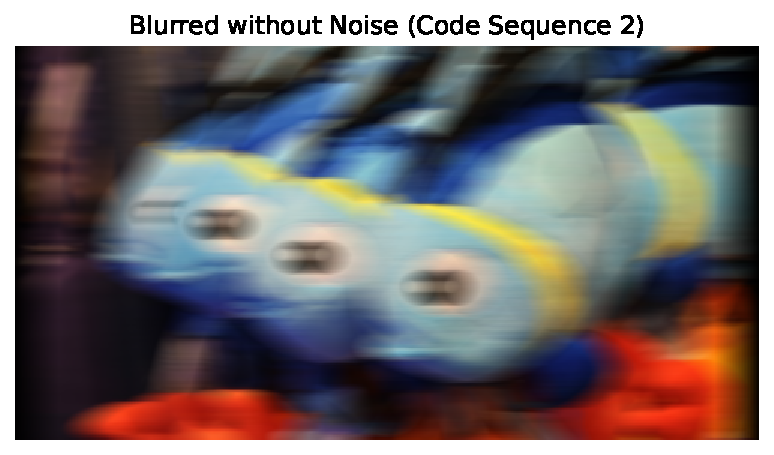
\includegraphics[width=1\linewidth]{../output/blurred_seq_2_without_noise.pdf}
							\caption{Blurred without noise(Code Sequence 2)}
							\label{fig:blurred_seq_2_without_noise}
						\end{subfigure}\\
						\begin{subfigure}[h]{1\linewidth}
							\centering
							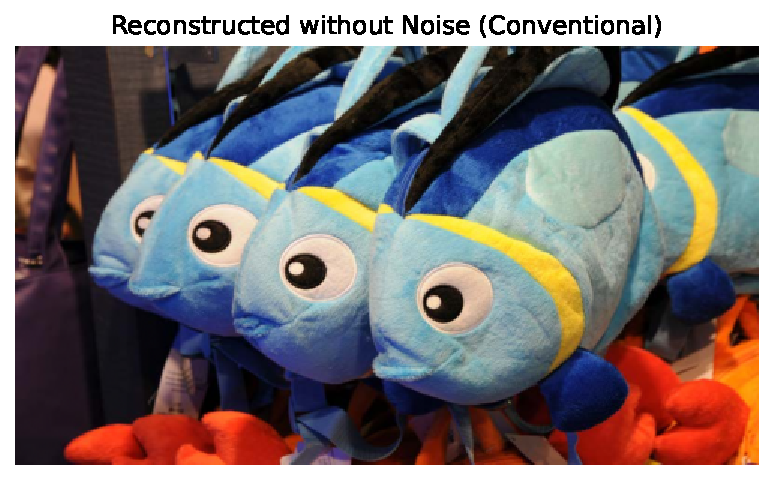
\includegraphics[width=1\linewidth]{../output/reconstructed_conventional_without_noise.pdf}
							\caption{Reconstructed without noise(Conventional)}
							\label{fig:reconstructed_conventioanl_without_noise}
						\end{subfigure} &
						\begin{subfigure}[h]{1\linewidth}
							\centering
							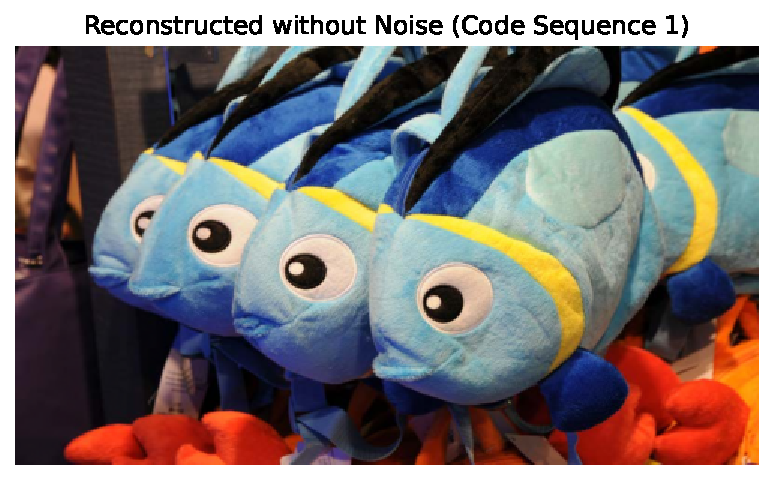
\includegraphics[width=1\linewidth]{../output/reconstructed_seq_1_without_noise.pdf}
							\caption{Reconstructed without noise(Code Sequence 1)}
							\label{fig:reconstructed_seq_1_without_noise}
						\end{subfigure} &
						\begin{subfigure}[h]{1\linewidth}
							\centering
							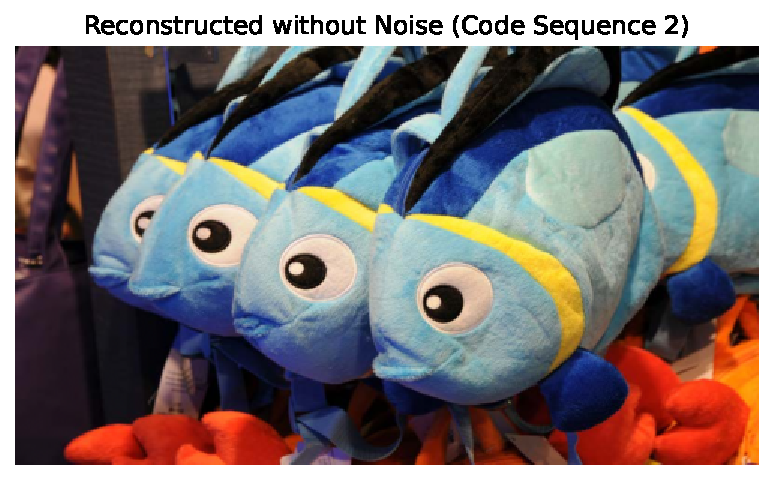
\includegraphics[width=1\linewidth]{../output/reconstructed_seq_2_without_noise.pdf}
							\caption{Reconstructed without noise(Code Sequence 2)}
							\label{fig:reconstructed_seq_2_without_noise}
						\end{subfigure}
					\end{tabular}
				}
				\caption{Blurred and reconstructed images without noise}
				\label{fig:blurred_reconstructed_without_noise}
			\end{figure}
		\end{enumerate}
		\item \textbf{Deblurring with motion-invariant photography}\\
		We are given images of the top view of a road scene \texttt{background.png }and a foreground moving object \texttt{redcar.png}.
		\begin{enumerate}
			\item \textbf{Static camera}\\
			We assume a static camera and model the car's velocity as $1$ pixels per second to the right (horizontal translation) relative to the camera. A blurred image is generated for an exposure time of $52$ seconds. To simulate this, we first create individual frames for each second, resulting in $52$ frames in total. For each frame, we apply the corresponding translation to the foreground object and then merge it with the background. During merging, all pixels with non-zero values in the foreground image are assigned the corresponding foreground pixel values, otherwise, they are assigned background pixel values. Finally, we average the $52$ frames to obtain the blurred image. The resulting images are shown in Figures \ref{fig:total_case_a}.
			\begin{figure}[H]
				\centering
				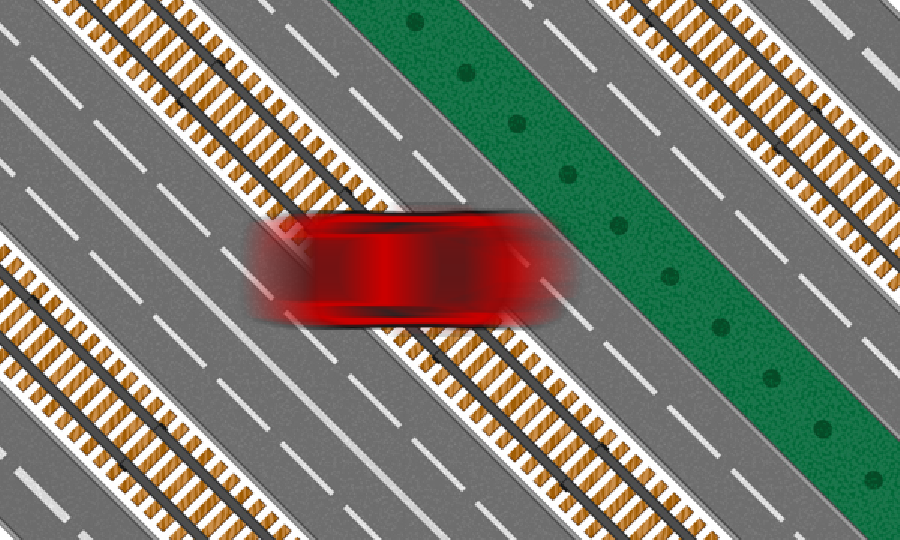
\includegraphics[width=0.7\linewidth]{../output/total_image_no_motion.pdf}
				\caption{Total image}
				\label{fig:total_case_a}
			\end{figure}
			\item \textbf{Motion-Invariant-Photography}\\
			We now consider the same scene captured using motion-invariant photography, where the camera itself moves during the exposure. The translational values of the static background, caused by camera motion at each second, are provided in \texttt{CameraT.mat}. In this case, we generate the blurred image with both camera and object motion for an exposure time of 53 seconds 
			(note that \texttt{CameraT} contains 53 entries, not 52).
			
			The process is as follows:
			
			\begin{itemize}
				\item For each second, we apply the camera-induced translations to the background image 
				and the relative translations to the moving object independently, and then merge them to form a single frame. 
				The relative motion of the object with respect to the moving camera is calculated as
				relative translation = static background translation due to camera - object translation
				
				\item Since the background translations caused by the camera are non-integer values, bilinear interpolation and target-to-source mapping are used to generate the translated frames.
				
				\item Finally, we average all 52 frames to obtain the motion-invariant blurred image.
			\end{itemize}
			The resulting output is shown in Figure \ref{fig:total_image_case_b}.
			\begin{figure}[H]
				\centering
				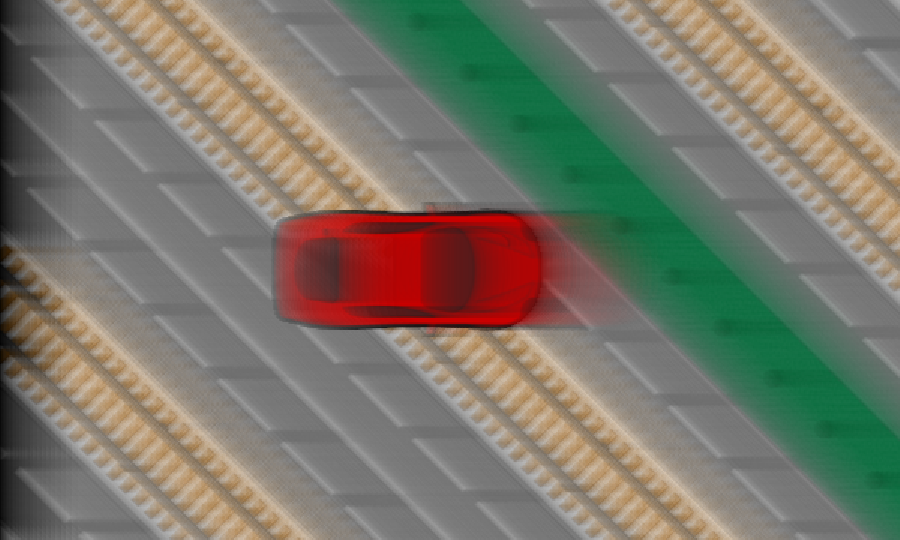
\includegraphics[width=0.7\linewidth]{../output/total_image_motion_invariant.pdf}
				\caption{Total image}
				\label{fig:total_image_case_b}
			\end{figure}
			\item \textbf{Comparison}\\
			In case (a), the foreground appears blurred while the background remains sharp, as both the background and the camera are stationary. In contrast, in case (b), both the foreground and background appear blurred because the camera is in motion, and the relative velocity between the camera and the foreground is non-zero.
		
			\item \textbf{PSF for Motion-Invariant Photography}\\
			We plot the PSF of the blurred image for the case of motion-invariant photography. If $x$ is the camera translation, the PSF weight at $x$ is $w(x)=1/x^2$ where $x=\{0.1,1,2\cdots52\}$ . We use $52$ instead of $51$ as given in the assignment to ensure that the shape of the blur matrix generated using it is valid for the blurred
			image. Figure \ref{fig:psf_motion_invariant} shows the normalized PSF 
			\begin{figure}[H]
				\centering
				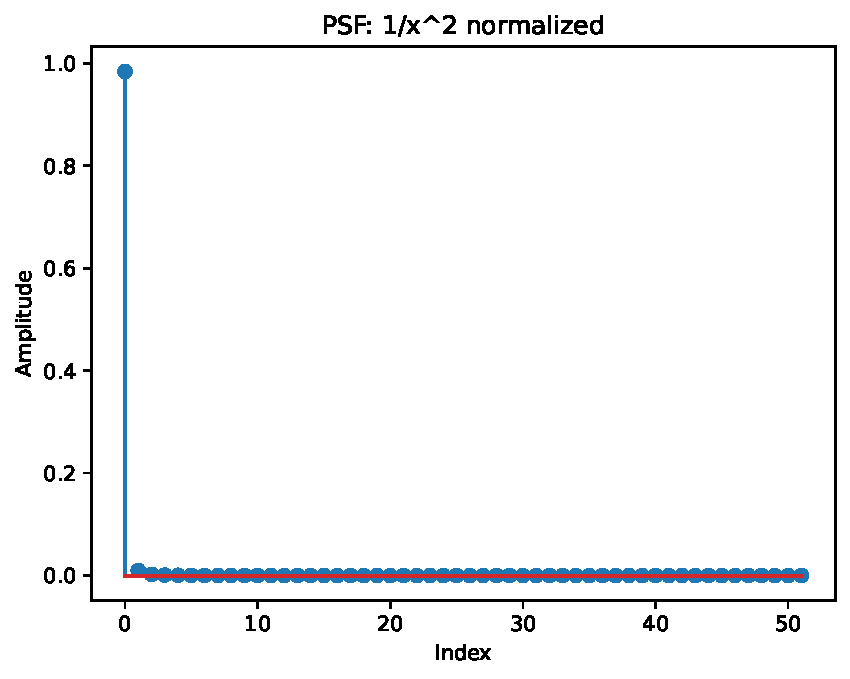
\includegraphics[width=0.6\linewidth]{../output/psf_motion_invariant.pdf}
				\caption{Normalized PSF for motion invariant photography}
				\label{fig:psf_motion_invariant}
			\end{figure}
			\item \textbf{Blur Matrix}\\
			We construct the blur matrices $A$ in the using the given PSF. Figure \ref{fig:toeplitz_matrix_motion_invariant}
			\begin{figure}[H]
				\centering
				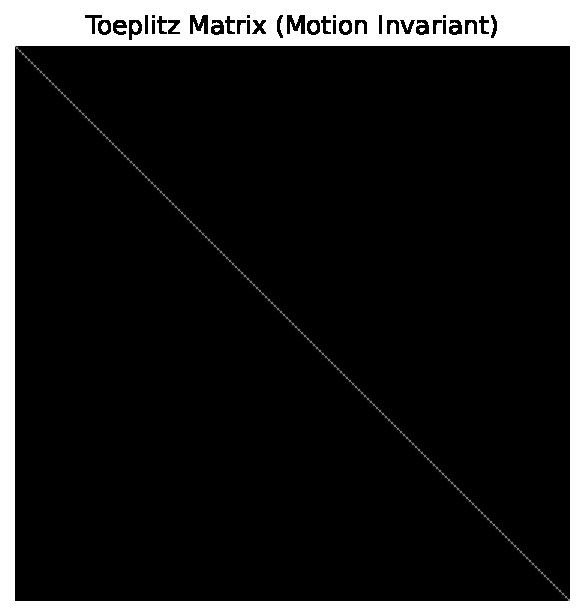
\includegraphics[width=0.6\linewidth]{../output/toeplitz_matrix_motion_invariant.pdf}
				\caption{Blur matrix(Motion Invariant)}
				\label{fig:toeplitz_matrix_motion_invariant}
			\end{figure}
			\item \textbf{Deblurred image}\\
			Similar to the conventional case, we estimate the deblurred image of Figure \ref{fig:total_image_case_b} using $A$ matrix. Figure \ref{fig:reconstructed_motion_invariant} show the reconstructed images obtained using the least squares method.
			\begin{figure}[H]
				\centering
				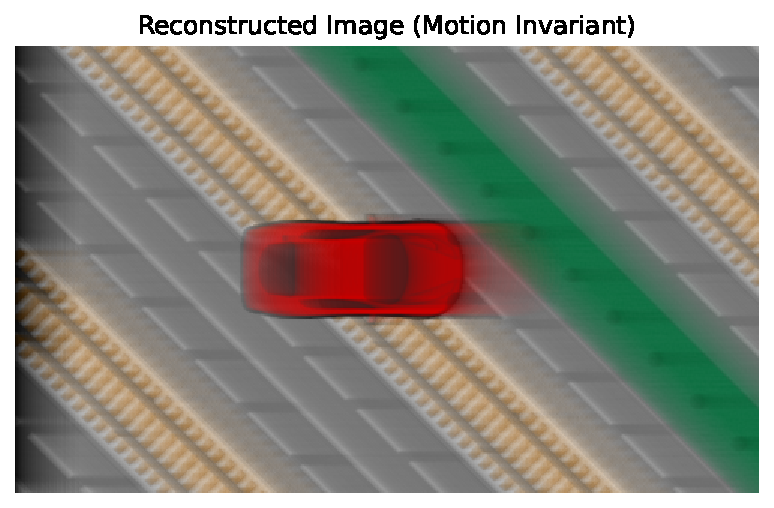
\includegraphics[width=0.7\linewidth]{../output/reconstructed_motion_invariant.pdf}
				\caption{Reconstructed(motion invariant)}
				\label{fig:reconstructed_motion_invariant}
			\end{figure}
			\end{enumerate}
	\end{enumerate}
\end{document}